\part{Elementos 1D}

\section{Elemento barra}
Uno puede pensar el elemento barra como un resorte que solo ejerce fuerza en la dirección en que apunta su eje local $x'$.
\begin{equation} \label{eq:matrizBarra}
\Mme{k'}_{\mathrm{barra}} = \begin{bmatrix}
X & -X \\ 
-X & X\\
\end{bmatrix}\begin{array}{c}
u_1\\
u_2 
\end{array} \qquad \text{donde}\qquad X=\frac{EA}{L}
\end{equation}
si se acopla la matriz a $\MK$ así como está solo otorga rigidez en la dirección $x$ global. Si se quiere modelar una barra en el plano $xy$ se tiene que rotar la barra según su orientación. Si el modelo es plano, osea solo se modelan $x$ e $y$ global, se puede rotar la barra como será visto en la sección \ref{sec:OrientacionBarras}. 

Para orientar una barra que se encuentra en el espacio se puede usar la matriz de rotación para una viga 3D con una leve modificación a la matriz de rigidez de la barra. Esta tiene que incluir todos los grados de libertad del problema! Es decir, la matriz $\Mme{k'}_{\mathrm{barra}}$ termina siendo de $12 \times 12$ para un problema de 6 grados de libertad por nodo.
\[
\mathbf{k}_{1,1}=\mathbf{k}_{7,7}=X, \qquad \mathbf{k}_{7,1}=\mathbf{k}_{1,7}=-X, \quad \text{las demás:} \quad \mathbf{k}_{i,j} = 0
\]
Un lector mosca ser dará cuenta que la matriz de rigidez de la viga Timoshenko 3-D (expresión \ref{eq:matrizRigidezTimoshenko}) es la generalización para todo elemento 1D: barras e incluso vigas en el plano.\footnote{Las formulaciones de vigas en el plano más comunes son de dos ($v$, $\theta$) y tres ($u$,$v$,$\theta$) grados de libertad por nodo.}

\subsection*{\textit{Bar element test}}
Llegado a este punto en la lectura, el autor se imagina que el lector debe estar ansioso por poner a prueba sus conocimientos. La figura \ref{fig:barpatch} describe un problema estático que se puede resolver con una breve análisis a mano alzada. Este tipo de problema se denomina \textit{patch test} o \textit{element test} porque sirve para ensayar la calidad del unión de elementos, el elemento en si, la aplicación de condiciones de borde y método de resolución. 
\begin{figure}[htb!]
	\centering
	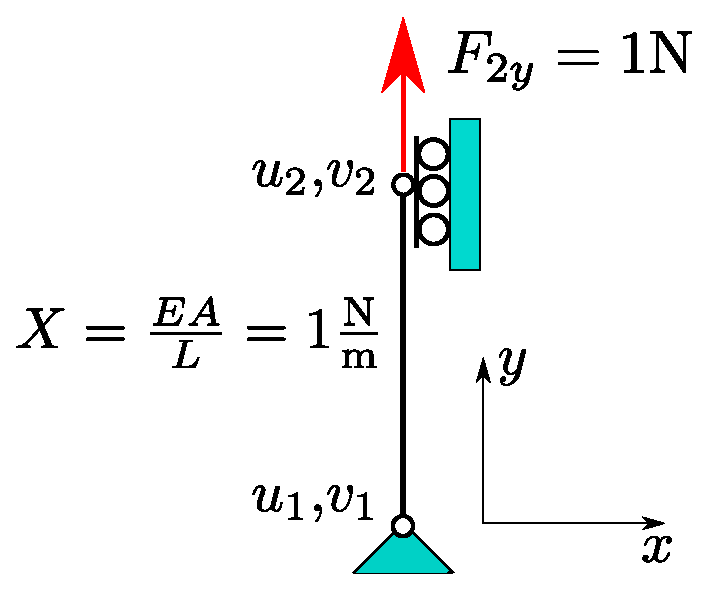
\includegraphics[width=0.4\textwidth]{fig/barpatch.eps}
	\caption{Un \textit{bar element test} para verificar un \textit{solver} de elementos finitos. $v_2=1$m.}
	\label{fig:barpatch}
\end{figure}

El \textit{bar element test} se puede mallar como un problema plano en el plano $xy$ con dos nodos ($x_1=y_1=x_2=0$, $y_2=1$m) y un elemento que los une. La rigidez del material entonces seria $EA=1$N. Se aplican las condiciones de borde detalladas en la figura: se restringen $u_1$,$v_1$ y $u_2$ y se resuelve el sistema para obtener $v_2$. Con este element test se verifica el método de resolución, la forma en que se rota la matriz de rigidez de la barra, la aplicación de condiciones de borde y el elemento en si. 


\section{Viga 3D de Timoshenko}
\begin{figure}[htb!]
	\centering
	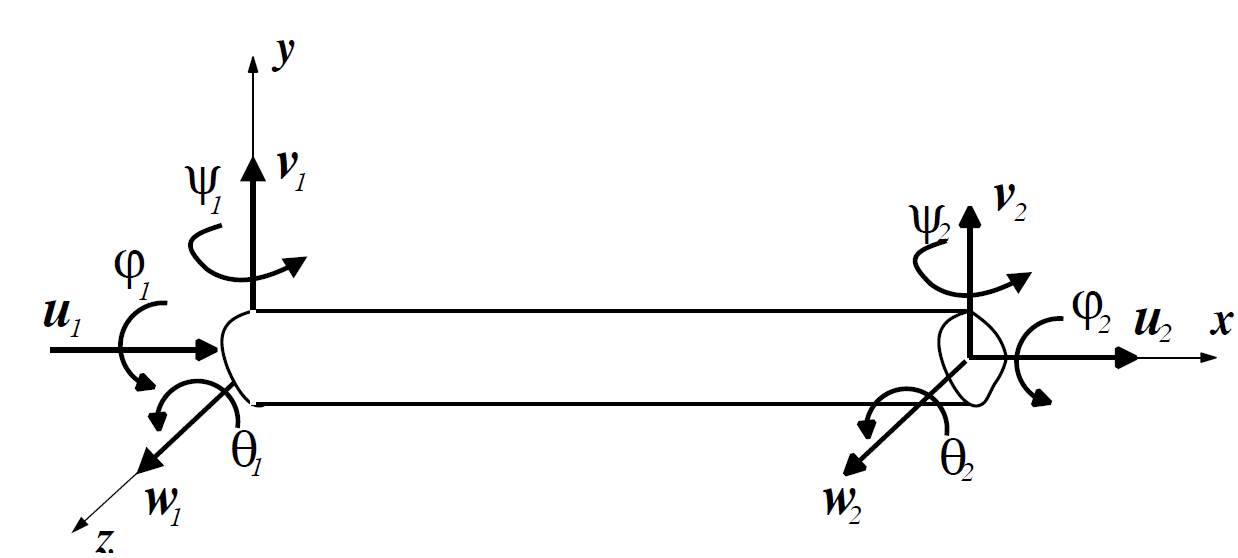
\includegraphics[width=0.6\textwidth]{fig/3dbeam.PNG}
	\caption{Grados de libertad (\textit{dof}) y coordenadas locales de una viga 3D de dos nodos y 6 dof por nodo.}
\end{figure}
La viga de Timoshenko 3D tiene las siguientes funciones de forma (forma eficiente tomada de \cite{luo2008efficient})
\[
\begin{cases}
\!\!\!\!\!
\begin{array}{l}
N_{1}=1-\xi \\
N_2 = \xi \\
\end{array}\Bigg\}\quad  \text{Funciones de forma para barras}\\
H_{v_{1}}=\beta_{y}\left(2 \xi^{3}-3 \xi^{2}+\alpha_{y} \xi+1-\alpha_{y}\right)\\
H_{v_{2}}=\beta_{y}\left(-2 \xi^{3}+3 \xi^{2}-\alpha_{y} \xi\right) \\
H_{w_{1}}=\beta_{z}\left(2 \xi^{3}-3 \xi^{2}+\alpha_{z} \xi+1-\alpha_{z}\right) \\
H_{w_{2}}=\beta_{z}\left(-2 \xi^{3}+3 \xi^{2}-\alpha_{z} \xi\right)\\
H_{\theta_{1}}=L \beta_{y}\left[\xi^{3}+\left(\frac{1}{2} \alpha_{y}-2\right) \xi^{2}+\left(1-\frac{1}{2} \alpha_{y}\right) \xi\right] \\
H_{\theta_{2}}=L \beta_{y}\left[\xi^{3}-\left(1+\frac{1}{2} \alpha_{y}\right) \xi^{2}+\left(\frac{1}{2} \alpha_{y}\right) \xi\right] \\
H_{\psi_{1}}=L \beta_{z}\left[\xi^{3}+\left(\frac{1}{2} \alpha_{z}-2\right) \xi^{2}+\left(1-\frac{1}{2} \alpha_{z}\right) \xi\right] \\
H_{\psi_{2}}=L \beta_{z}\left[\xi^{3}-\left(1+\frac{1}{2} \alpha_{z}\right) \xi^{2}+\left(\frac{1}{2} \alpha_{z}\right) \xi\right] \\
G_{v_{1}}=\frac{6 \beta_{y}}{L}\left(\xi^{2}-\xi\right) \\
G_{v_{2}}=\frac{6 \beta_{y}}{L}\left(-\xi^{2}+\xi\right) \\
G_{w_{1}}=\frac{6 \beta_{z}}{L}\left(\xi^{2}-\xi\right) \\
G_{w_{2}}=\frac{6 \beta_{z}}{L}\left(-\xi^{2}+\xi\right) \\
G_{\theta_{1}}=\beta_{y}\left[3 \xi^{2}+\left(\alpha_{y}-4\right) \xi+1-\alpha_{y}\right] \\
G_{\theta_{2}}=\beta_{y}\left[3 \xi^{2}-\left(\alpha_{y}+2\right) \xi\right] \\
G_{\psi_{1}}=\beta_{z}\left[3 \xi^{2}+\left(\alpha_{z}-4\right) \xi+1-\alpha_{z}\right] \\
G_{\psi_{2}}=\beta_{z}\left[3 \xi^{2}-\left(\alpha_{z}+2\right) \xi\right]
\end{cases}
\]
donde $x'$ es la coordenada local sobre la viga:
\[
\xi=\frac{x'}{L}, \qquad \alpha_{y}=\frac{12 E I_{y}}{k G A L^{2}}, \qquad \beta_{y}=\frac{1}{1-\alpha_{y}}, \qquad \alpha_{z}=\frac{12 E I_{z}}{k G A L^{2}},\qquad \beta_{z}=\frac{1}{1-\alpha_{z}}
\]
donde $k$ es el \textbf{factor de corrección por corte}\footnote{Ideado por Timoshenko en 1921 para permitir un mejor cálculo de las frecuencias naturales \cite{dong2010much}.} y depende de la sección y del modulo de Poisson $\nu$. Algunos valores en la tabla \ref{tab:kcorrectionfactor} del anexo.

Estas funciones de forma interpolan los desplazamientos sobre la viga:

\begin{equation} \label{eq:interpolacionFuncForma1D}
\begin{cases}
u=N_{1} u_{1}+N_{2} u_{2} \\
v=H_{v_{1}} v_{1}+H_{\theta_{1}} \theta_{1}+H_{v_{2}} v_{2}+H_{\theta_{2}} \theta_{2} \\
w=H_{w_{1}} w_{1}+H_{\psi_{1}} \psi_{1}+H_{w_{2}} w_{2}+H_{\psi_{2}} \psi_{2} \\
\varphi=N_{1} \varphi_{1}+N_{2} \varphi_{2} \\
\theta=G_{v_{1}} v_{1}+G_{\theta_{1}} \theta_{1}+G_{v_{2}} v_{2}+G_{\theta_{2}} \theta_{2} \\
\psi=G_{w_{1}} w_{1}+G_{\psi_{1}} \psi_{1}+G_{w_{2}} w_{2}+G_{\psi_{2}} \psi_{2}
\end{cases}
\end{equation} 



para luego calcular los esfuerzos usando las mismas formulas vistas en estática y resistencia de materiales.
\begin{align*}
M_{z}&=E I_{z} \frac{\di^{2} v}{\di x^{2}}, \qquad V_{y}=\frac{\di M_{z}}{\di x}=E I_{z} \frac{\di^{3} v}{\di x^{3}}, \qquad N_x=A E \frac{u_{2}-u_{1}}{L} \\
\qquad T&=G J_T \frac{\varphi_{2}-\varphi_{1}}{L}, \qquad M_{y}=E I_{y} \frac{\di^{2} w}{\di x^{2}}, \qquad V_{z}=E I_{y} \frac{\di^{3} w}{\di x^{3}}
\end{align*}
donde $J_T$ es la constante torsional de la viga y $A$ es la sección. \footnote{La constante torsional $J_T$ es igual a $I_p$ para secciones de viga circulares. Para perfiles abiertos de paredes delgadas, como por ejemplo un perfil doble T o un perfil `C', $J_T$ es mucho mas chico que $I_p$.}

La matriz de rigidez se puede obtener\footnote{Para una viga uniforme con sección simétrica y de  material en su rango elástico.} integrando analíticamente a la funciones de forma mencionadas anteriormente sobre el largo de la viga. En este documento no se va tratar la matriz de rigidez que resulta de dicha integración. Se presenta al lector la matriz de rigidez de una viga Timoshenko 3D clásica \cite{cook2007concepts}:

\begin{equation}\label{eq:matrizRigidezTimoshenko} \Mme{k'}_{\mathrm{1D}} = \left[\begin{array}{cccccccccccc} X & 0 & 0 & 0 & 0 & 0 & -X & 0 & 0 & 0 & 0 & 0\\ 0 & Y_{1} & 0 & 0 & 0 & Y_{2} & 0 & -Y_{1} & 0 & 0 & 0 & Y_{2}\\ 0 & 0 & Z_{1} & 0 & -Z_{2} & 0 & 0 & 0 & -Z_{1} & 0 & -Z_{2} & 0\\ 0 & 0 & 0 & S & 0 & 0 & 0 & 0 & 0 & -S & 0 & 0\\ 0 & 0 & -Z_{2} & 0 & Z_{3} & 0 & 0 & 0 & Z_{2} & 0 & Z_{4} & 0\\ 0 & Y_{2} & 0 & 0 & 0 & Y_{3} & 0 & -Y_{2} & 0 & 0 & 0 & Y_{4}\\ -X & 0 & 0 & 0 & 0 & 0 & X & 0 & 0 & 0 & 0 & 0\\ 0 & -Y_{1} & 0 & 0 & 0 & -Y_{2} & 0 & Y_{1} & 0 & 0 & 0 & -Y_{2}\\ 0 & 0 & -Z_{1} & 0 & Z_{2} & 0 & 0 & 0 & Z_{1} & 0 & Z_{2} & 0\\ 0 & 0 & 0 & -S & 0 & 0 & 0 & 0 & 0 & S & 0 & 0\\ 0 & 0 & -Z_{2} & 0 & Z_{4} & 0 & 0 & 0 & Z_{2} & 0 & Z_{3} & 0\\ 0 & Y_{2} & 0 & 0 & 0 & Y_{4} & 0 & -Y_{2} & 0 & 0 & 0 & Y_{3} \end{array}\right]\begin{array}{c}
u_1\\
v_1 \\
w_1 \\
\varphi_1 \\
\psi_1 \\
\theta_1 \\
u_2\\
v_2 \\
w_2 \\
\varphi_2 \\
\psi_2 \\
\theta_2 
\end{array}
\end{equation} 
donde  
\begin{align*}
X&=\frac{AE}{L}, \qquad Y_4 = \frac{2EI_z}{L}, \qquad Y_3 = 2Y_4, \qquad Y_2 = \frac{3Y_4}{L} ,\qquad Y_1 = \frac{2Y_2}{L} \\
Z_4 &= \frac{2EI_y}{L}, \qquad Z_3=2Z_4, \qquad Z_2 = \frac{2Z_4}{L}, \qquad Z_1 = \frac{2Z_2}{L}, \qquad S = \frac{G J_T}{L}
\end{align*}

\subsection*{Rótulas}

\begin{figure}[htb!]
	\centering
	\begin{subfigure}{0.49\textwidth}
		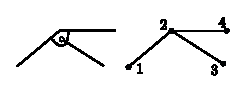
\includegraphics[width=\linewidth]{fig/rotulaexample.eps}
		\caption{Una unión rotulada y una posible discretización.}
		\label{fig:rotulaexample}
	\end{subfigure}
	\begin{subfigure}{0.49\textwidth}
		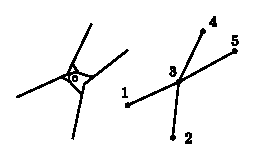
\includegraphics[width=\linewidth]{fig/rotulaexample2.eps}
		\caption{Dos sistemas de vigas unidos por una rótula y una posible discretización.}
		\label{fig:rotulaexample2}
	\end{subfigure}
	\caption{}
\end{figure}



Las uniones rotuladas permiten que ciertos elementos giren libremente manteniendo rigidez ante la rotación de otros elementos. El primer paso consiste en \textbf{desacoplar} el/los\footnote{Suponiendo que la figura \ref{fig:rotulaexample} está contenida en el plano $xy$: el giro a desacoplar sería en $z$ ($\theta$) dado la geometría de la rótula.} giro/s del elemento rotulado. Esto se logra generando un nuevo grado de libertad para cada giro desacoplado, el cual \textit{no pertenece a ningún nodo}, un \textit{nodeless dof}. Este nuevo dof se puede introducir al final de la matriz de rigidez para no estropear el mapeo de dof visto anteriormente. Al momento de acoplar la rigidez del elemento a la matriz de rigidez global la matriz \texttt{elemdof} (sección \ref{sec:dofmapping}) tiene que mostrar este cambio con los dof desacoplados. Para el caso de la figura \ref{fig:rotulaexample} con grados de libertad $u,v,\theta$ por nodo:

\begin{equation*} \label{eq:elemdofParaRotulaEjemplo}
\texttt{elementos} = \begin{bmatrix}
1 & 2  \\
2 & 4 \\
3 & 2\\
\end{bmatrix},
\qquad
\texttt{elemdof} = \begin{bmatrix}
1 & 2 & 3 & 4 & 5 & 6 \\
4 & 5 & 6 & 10 & 11 & 12  \\
7 & 8 & 9 & 4 & 5 & 13 \\
\end{bmatrix}
\end{equation*}
note que el elemento rotulado comparte los desplazamientos $u,v$ sobre el nodo 2 (dof 4 y 5) con los otros dos elementos pero tiene su giro $\theta$ desacoplado.

\textit{¿Como quedaría la matriz \texttt{elemdof} del sistema de la figura \ref{fig:rotulaexample2}?}


\section{Orientación de elementos 1D} \label{sec:OrientacionElementos}
Los elementos detallados en la sección anterior están acostados sobre el eje $x$. Para orientar un elemento en el espacio se tiene que empezar de hablar de una \textit{matriz de rotación} $\Mme{T}$.

\begin{equation} \label{eq:rotacionElemento}
\Mk_{\mathrm{rotada}}= \Mme{T}^T \Mme{k'} \Mme{T}
\end{equation}
donde $\Mme{k'} $ es la matriz de rigidez local del elemento 1D antes de ser rotado. Luego de ser rotada la matriz puede ser acoplada a la rigidez global del sistema $\MK$.

Cabe agregar que los desplazamientos relacionados con el sistema global corresponden a los ejes globales. Para obtener los desplazamientos locales de los elementos se tienen que rotar estos también!

\begin{equation} \label{eq:rotacionDesplazamientos}
\Cme{d'}= \Mme{T} \Cme{d}  
\end{equation}
donde $\Cme{d'}$ son los desplazamientos del elemento en las coordenadas locales. Obtener $\Cme{d'}$ resulta útil al momento de querer calcular las fuerzas\footnote{El signo negativo es para obtener las fuerzas \textbf{internas} actuando en el elemento.} locales del elemento: \( \Mme{k'}\Cme{d'}= - \Cme{r'} \) o para interpolar los desplazamientos usando las expresiones en \eqref{eq:interpolacionFuncForma1D}.

\subsection*{Orientación de barras en el plano} \label{sec:OrientacionBarras}
La matriz de rigidez de una barra es definida horizontal. Esto significa que toda la rigidez está en $x$.

Una barra rotada $\phi$ grados va tener una nueva rigidez en el eje global $x$, e incluso puede no tener rigidez si se rota 90 grados.

La matriz transformación de una barra en el plano está dada por 

\[
\Mme{T}_{\mathrm{Barra}}= \begin{bmatrix}
\cos \phi & 0 \\
\sin \phi & 0 \\
0 & \cos \phi \\
0 & \sin \phi
\end{bmatrix}
\]

\subsection*{Orientación de vigas en el espacio}
Para orientar una viga se tiene que aportar más información que para una barra. Mientras que una barra se puede orientar con el simple input de sus nodos, la viga de Timoshenko necesita orientar su eje $y'$ además de su eje $x'$ .

Algunos programas como \Adina, por ejemplo, permiten al usuario especificar un nodo auxiliar o un vector auxiliar que apunta en la dirección en la cual se desea que la viga tenga su eje $y'$. 

Supongamos que elegimos este vector auxiliar $s_y=[0,1,0]$.\footnote{\textbf{Ser cauteloso al elegir el vector $s_y$ para que bajo ninguna circunstancia quede colineal al eje $x'$ del elemento. Esto causará problemas insanables.}} Esto nos va dar el mayor momento ante la flexión para una carga en $y$ global (suponiendo que $I_z>I_y$).

Para hallar la matriz de transformación $\Mme{T}$ debemos buscar los cosenos directores de nuestra viga en el espacio. Una vez que obtenemos el versor de orientación\footnote{Es el que resulta de la resta entre los nodos del elemento.} $\versor{v}_x$ es trivial obtener $\versor{v}_z$
\[
\versor{v}_z = \frac{\versor{v}_x\times s_y}{||\versor{v}_x\times s_y||}
\]
Luego de armar los versores $\versor{v}_x$, $\versor{v}_y$, $\versor{v}_z$ se define la matriz de los cosenos directores $\pmb{\lambda}$

\[
\pmb{\lambda} = \begin{bmatrix}
\versor{v}_x \\
\versor{v}_y \\
\versor{v}_z 
\end{bmatrix}_{3\times3}
\]

La matriz de transformación entonces es

\begin{equation}
\Mme{T}_{\mathrm{1D}}=\begin{bmatrix}
\pmb{\lambda} & &\cdots & 0 \\
&\pmb{\lambda} &  &\vdots \\
\vdots & &\pmb{\lambda} & \\
0 &\cdots & & \pmb{\lambda}
\end{bmatrix}_{12\times 12}
\end{equation}


\section{Cargas}
\subsection*{Cargas Consistentes}
Una carga distribuida en $-y'$ sobre una viga que está fija en sus extremos tiene las cargas nodales

\begin{equation} \label{eq:CargaDistribuidaElemento}
\Cme{r'} = \begin{Bmatrix}
0 \\
-qL/2 \\
0\\
0\\
0\\
-qL^2/12\\
0\\
-qL/2 \\
0\\
0\\
0\\
qL^2/12
\end{Bmatrix}
\qquad q \text{  en } \left[\frac{\text{Fuerza}}{\text{Longitud}} \right]
\end{equation}
estas son las cargas \textbf{\textit{consistentes}} porque toman en cuenta los momentos generados. Si se omiten los momentos se llaman \textit{cargas reducidas}.

Si la viga tiene una carga distribuida sobre su eje $y'$ local pero está arbitrariamente orientada se pueden obtener las cargas globales a aplicar sobre los nodos del elemento usando la matriz de rotación usada para orientar el elemento

\begin{equation}
\Cme{r}= \Mme{T}^T \Cme{r'}
\end{equation}
usando $\Cme{r'}$ de \eqref{eq:CargaDistribuidaElemento}. Si la carga no está sobre el eje $y'$ de la viga, se deberá usar una matriz de rotación diferente, o cambiar el vector de cargas predefinido. \textit{¿Como aplicaría un par torsor a una viga arbitrariamente orientada?}
\section{Ejercicios}
\subsection*{Pórticos}

\begin{figure}[htb!]
	\centering
	\begin{subfigure}{0.49\linewidth}
		\centering
		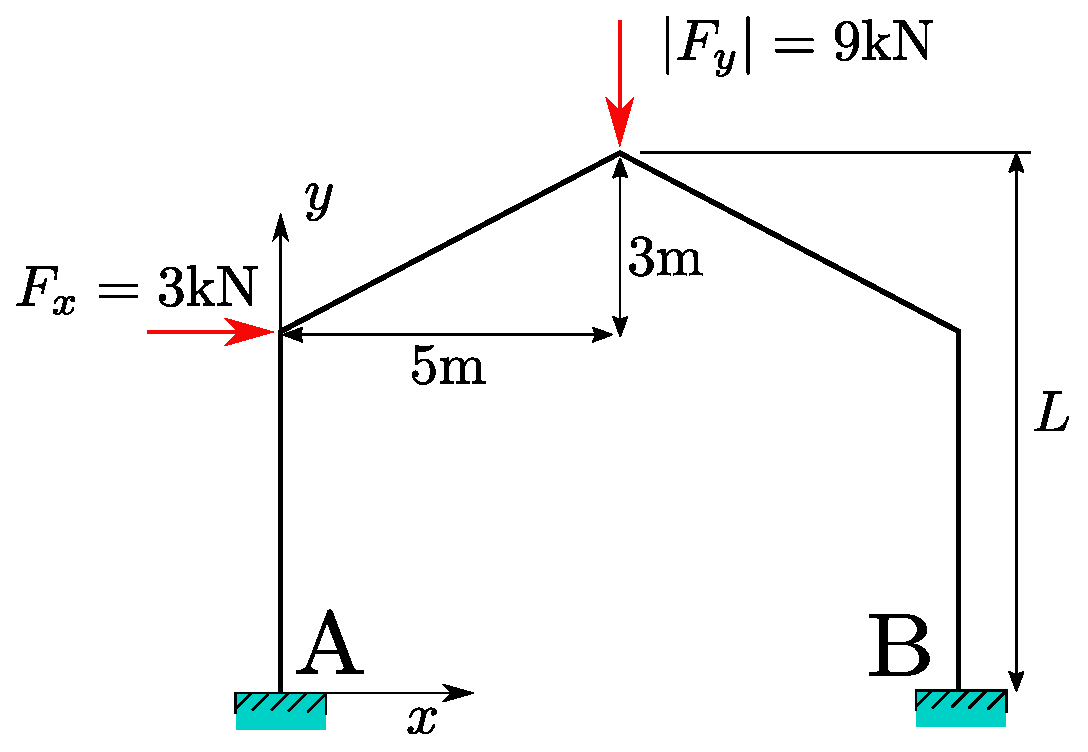
\includegraphics[width=1\textwidth]{fig/ej1viga.eps}
		\caption{Pórtico de altura $L$ a escala para el problema \ref{ej:probvigaaltura} }
		\label{fig:ej1viga}
	\end{subfigure}
	\begin{subfigure}{0.49\linewidth}
		\centering
		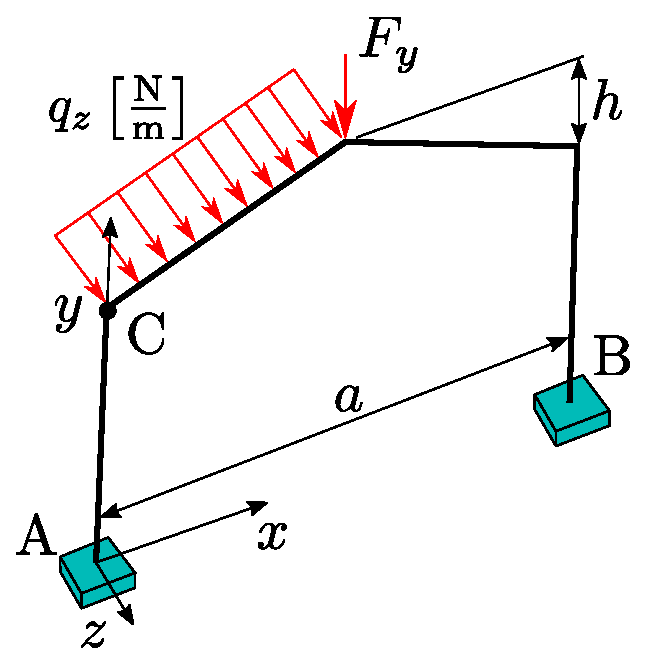
\includegraphics[width=.663\textwidth]{fig/ej2viga.eps}
		\caption{Pórtico con una carga distribuida en dirección $z$}
		\label{fig:ej2viga}
	\end{subfigure}
	\caption{}
	\label{fig:ejPorticos}
\end{figure}
\begin{enumerate}
	\item Para la figura \ref{fig:ej1viga} efectuar un modelo matemático y luego discretizar para resolver:
	\begin{enumerate}
		\item Verificar que para el caso dado con $F_x=0$ las reacciones en $y$ de los empotramientos son $\frac{F_y}{2}$.
		\item Se diseño el pórtico con una altura $L=7$ metros con perfiles IPN 160. Un análisis preliminar de una consultora sugiere que el punto superior supera los desplazamientos máximos permitidos de $d_{\max}=15$mm. Verificar.\label{ej:porticoVerificarConsultora}
		\item ¿Que altura debería el pórtico así el punto superior no se desplaza mas que $26.7$mm? Usar perfil IPB\footnote{Se puede buscar también como perfil HEB.} 120. ¿Es esta la configuración de la figura \ref{fig:ej1viga}? (\textit{hint:} si lo es)\label{ej:probvigaaltura}
	\end{enumerate}
	\item Para la figura \ref{fig:ej2viga} considerar perfiles HEB 340. 
	\begin{enumerate}
		\item Las reacciones considerando $a=12$m, $h=2$m  y una altura de $8$m. $q_z=500$ y $F_y=20$kN. \label{ej:reaccionportico3D}
		\item ¿Que orientación de vigas es favorable para reducir el desplazamiento del punto C?\label{ej:favorableportico3D} 
	\end{enumerate}
\end{enumerate}
Algunas Respuestas considerando $E=200$GPa:
\begin{itemize}
	\item[\ref{ej:porticoVerificarConsultora})]$d=0,0155$m, $\Cme{R_A}\approx\{1,1;\ms4,1;\ms-1,28\}$ kN o kNm
	
	\item[\ref{ej:reaccionportico3D})] $\Cme{R_B}\approx
	\{-6,2;\ms    10;\ms   -0,79;\ms   -0,64;\ms   -6,4;\ms   -0,5;\ms   16\}$ kN o kNm, con cargas reducidas
	
	\item[\ref{ej:favorableportico3D})] $d_{\mathrm{C}}=2,38$mm
	
\end{itemize}
\clearpage